%% LyX 2.0.2 created this file.  For more info, see http://www.lyx.org/.
%% Do not edit unless you really know what you are doing.
\documentclass[english]{article}
\usepackage[T1]{fontenc}
\usepackage[latin9]{inputenc}
\usepackage{geometry}
\usepackage{subfig}
\usepackage{graphicx}
\DeclareGraphicsExtensions{.pdf,.png,.jpg}
\geometry{verbose,tmargin=4cm,bmargin=4cm,lmargin=4cm,rmargin=4cm}
\usepackage{babel}
\usepackage{setspace}
\doublespacing
\begin{document}
\begin{center}
\section*{Final Project: Optimization for Shopping Cart Batch Return Times}
\subsection*{Adel Amodwala, 997064527}
\end{center}

\section*{Introduction}
Imagine driving up to a supermarket and being greeted outside the front doors by an empty space where the shopping carts used to be: You either now have to wait for a cart to return, reduce your shopping list, or be prepared to use your juggling skills. In any case, the main problem you as a customer faces is the inconvenience of not having a cart with you while you shop. On the other hand, as the manager of a supermarket, you might be faced with customer complaints, reduced sales (since people might opt to reduce their shopping lists), or more clean-ups and breakage (when people start juggling with grocery items). Even worse, if repeat customers are irritated by a scarcity of carts, they may shop at other stores more frequently or stop coming to your store all together. This poses a larger loss to revenues, however it does reduce the number of people which visit the store, hence the demand of carts will eventually be met by the (though scarce) supply of carts. Although this does solve the problem for the customers that get lucky enough to usually get carts and decide to continue shopping, as the manager of the store, this hardly seems like the ideal solution to keep customers returning to your store and maximizing your overall revenues. So what can the manager do?

The answer is simple: make more carts available to customers! The direct way of doing this is purchasing more carts. While this does include a cost to the store, one might be able to justify spedning money to keep customers returning rather them leaving for the lack of shopping carts. Naturally one might ask how many carts will be required to meet customer demand, and based on the arrival and departure rates of customers (assuming the store manages to collect the data over a few weeks every season), be able to determine such a number. However, the arrival and departure rates of customers doesn't tell us much about the arrival and departure rates of shopping carts from their home (i.e. their deployment base): some customers might not use carts and among those that do, many might be too lazy or distracted to return used carts (e.g. leaving them in the parking lot or somewhere in the store during or after usage). So the store could possibly purchase an enormous amounts of shopping carts before they are rid of the scarcity problem while incurring a large amount of cost to supply said carts. 

A more efficient workaround all supermarkets have adopted is having certain employees collect abandoned shopping carts from the store premises and returning them. The time interval between these 'batch returns' depends on the number of trolleys that are abandoned: if there are no abandoned carts, the workers do not return any of them, and if there are a few carts, the workers might ignore them, but if there are a lot of abandoned carts, then the workers would return them as soon as possible. This method however requires the workers to be vigilant for the most part. A better method of determining optimal batch return times might be to simulate a supermarket environment and check, given arrival and departure rates of customers that use carts, what the largest possible time interval the manager can set so that employees don't need to be vigilant and can more or less have a 'schedule' for returning the carts (e.g. approximately every hour or so, perhaps a little earlier or later). We will develop a more sound rationale for finding an optimal return time strategy later on in the paper.

Next, we will define our problem more concretely and set up a basic environment where only arrival and departure rates of cart users as well as the number of carts are considered parameters (obviously in reality we can't control arrival and departure rates of the customers, however since we are not assuming any fixed rate based on collected data, we are free to study the behaviour of different rates and number of carts available to customers). Following our simple model, we will introduce the use of batches and try to find an optimal return time which leaves a good number of carts for arriving customers to pick up.

\section*{A Simple Environment without Batch Returns}

Suppose that 'home' (cart deployment base) contains $N$ queues of carts, each containing $M$ carts initially (and at most). We can safely assume that the arrival rates of customers that are interested in using carts follows a Poisson Point Process with some rate $\gamma$. Since we are interested in the perspective of the shopping carts, this $almost$ translates to the following: the waiting time between departures of carts is $Exponential(\gamma)$. This statement is incomplete since there is something to be said about the spatial arrangement of the carts each time a customer arrives: in this model, we assume that when a customer stands in front of home, they are most likely to grab a cart closest to them (i.e. they will get a cart from the queue with the largest number of carts). However, sometimes there are obstacles to get such a cart (e.g. the cart is stuck and unable to come out, or there are physical hurdles to get to the cart), hence not all carts are given equal weight with respect to selection, and the weights are given to carts in terms of the number of carts in their respective queues. The queue which the cart will be taken from is sampled using the weights.

For example, if we initially have three queues with five carts each (i.e. $N=3,M=5$), then at state $t$, if queue 1 has 4 carts, queue 2 has 2 carts, and queue 3 has 3 carts, then the last cart (the one facing the customer) of queue 1 will have the highest weight as opposed to the last carts of queues 2 and 3 respectively.

More formally, we have queues $Q_i, i\in\{1,...,N\}$, and let $|Q_{i}^{(t)}|$=\# of carts in queue $i$ at time $t\geq0$, and by assumption $|Q_{i}^{(t)}|\in\{0,...,M\}$. Then the departure weights for the last cart in $Q_{i}^{(t)}$ at time $t$ is given by 
\[
w_{d_i}^{(t)}=\frac{|Q_{i}^{(t)}|}{\sum_{j=1}^{N}|Q_{j}^{(t)}|}, i \in \{ 1,..., N\}.
\]
As for the rate at which carts arrive, we make the following assumptions (and their justifications): Customers are served (i.e. the time it takes for them to shop) with exponential times (say of rate $\alpha$). Furthermore, customers are not necessarily 'well-behaved', i.e. they don't always return the cart they've used to home. Therefore, we have that, again $almost$, the interarrival times of shopping carts is $Exponential(\alpha)$. Furthermore, we again consider the spatial arrangement of the carts and how customers are likely to return them: we assume that customers are inherently efficiency seeking (i.e. lazy) so that they will expend as little effort as possible to return their cart. This would imply that customers always give more weight to queues that have more carts in them, which makes them 'closer' so they have to take fewer steps to return their cart. However, there would be a physical barrier from returning carts to queues that already have $M$ carts in them (and we safely assume the barrier does not prevent customers to take carts away). Futhermore, we don't imagine this to always be the case, again perhaps due to physical limtations/barriers, and hence the queue chosen at time $t$ will be random with the weights, for $Q_{i}^{(t)}$ as
\[
w_{a_i}^{(t)}=I(i \in G^{(t)} \neq \emptyset) \{\frac{|Q_{i}^{(t)}|I( T^{(t)} \neq 0 )}{ T^{(t)}} + \frac{I( T^{(t)} = 0)}{|G^{(t)}|}\}
\]
where
\[
G^{(t)}=\{i:|Q_{i}^{(t)}| \leq M-1, \forall  i \in \{ 1,..., N\} \},  
\]
\[
T^{(t)} = \sum_{j\in G^{(t)}}^{N}|Q_{j}^{(t)}|
\]
And $I(A)$ is the indicator function of the event $A$. Here, we give zero weight to full queues, hence accounting for the 'physical block if a queue already has $M$ carts'. If all of the queues in $G^{(t)}$ were empty, then they would be given an equal chance to recieve an arriving cart since the customer would be indifferent (based on the simplifying assumption that if all the available queues are empty, the spatial arrangement no longer matters, hence randomly sampled according to equiprobable weights). On the other hand, if there are queues with non-zero sizes, then we give higher weight to those with more carts.

\subsection*{Some Simulation Results}
\subsubsection*{Code Implementation and Challenges}
I had originally designed a quasi-object oriented environment in R where carts were to be data frames containing original indices in matrix form (so the first cart facing the customer from $Q_j$ would have indices $(j,M))$, time of departure, and expected arrival time. Furthermore, home would be a list object containing other lists, i.e. the queues as stacks, whose elements were the cart data frames. Unfortunately, this design proved to be unstable as some elements of the data frame would disappear and the code would break down. Therefore, the code was implemented in a neater fasion in Python where I was able to use Node objects for carts and stacks for our queues at home, and a dictionary/hash table for home itself. This allowed me to write methods relating specifically to each data type, rather than depending on some pre-existing function and having to worry about code failure.

The coding for each data type is given in Part A of the Appendix. For the carts, we use the Node data structure where we can record the indices, time cart was taken out by a customer (timestamp), the expected time to return for the cart (returnt), and a boolean to identify if that cart is currently out of home (True) or not (False). Furthermore, we want to be able to compare carts for equality, i.e. if one cart object is the same based on its indices. There is also a method for string representation where we get all the information about the cart (indices, timestamp, returntime, out).

For the queues in home, we essentially have a list that can contain several node/cart objects. The queues are defined as stacks with a Last In First Out (LIFO) treatment for nodes. Finally, home is a Matrix data type (it's just a name as the data type is a dictionary of queues), where each key of the dictionary maps to a queue. For instance, the $i^{th}$ queue has key $i \in \{ 1,...,N\}$ with mapped value being a stack object (the queue) containing nodes (carts). Each stack object has methods to pop the last element, push in a new element at the end, a length method (size) to check the number of nodes in the queue, a remove method to remove a node at some index in the stack, and a find method to search for a given node object. Many of these methods will be used in our more complicated model when we build stacks for carts that are out and carts that have been abandoned, but for now we will use the Matrix type to create home (X) and a stack for carts that have been taken out (Out).

The helper functions we've used include the computation of departure weights for the last carts in each non-empty queue (the carts facing the customer), arrival weights for non-full queues (i.e. queues with size less than $M$), a function that returns indices based on such weights, and some functions for creating new arrival and departure times of the carts. We also have a function called outweights that computes the weights of the carts that have been taken out by giving the largest weight to the cart with the smallest return time. More precisely, we have
\[
w_{j}^{(t)} = I(|Out^{(t)}|>0) \frac{\frac{1}{cart.returnt_j}}{\sum_{k=1}^{|Out^{(t)}|}\frac{1}{cart.returnt_k}}
\]
Where $Out^{(t)}$ is the Out stack at time $t$, $|Out^{(t)}| =\# $ of elements in $Out$ at time t, and $cart.returnt_k>0$ is the return time of the $k^{th}$ cart in the $Out$ stack. The reason why we sample from $Out$ rather than deterministically select the smallest return time is to factor for randomness that occurs with certain customers that might take more or less time with their shopping than anticipated.

\subsubsection*{Simulation Code and Comparisions}
The simulation code is provided in Part C of the Appendix. We begin by initializing home (X), Out (for carts that have been taken out), and Aban (for carts that have been abandoned). In the simple environment, there are no abandoned carts so this stack will be left alone. Next we initialize a few parameters such as the TARGETTIME (overall run of the Monte Carlo simulation), MAXGRAPH (which is the same as $M$), whether we include batch returns (set to False for the simple environment), a new time to first departure and a time to first arrival (since all the carts are already home, there is to be no new arrival until the first cart has departed), timeremaining which counts down time until the simulation is over, thetimesQ which is a dictionary with keys being the queue index whose values are lists that record the time spent in a paricular state (i.e. it will record how long the chain has spent time in state $Q_{i}^{(t)} = s \in \{ 0,...,M\}$ for each $Q_{i} \in X$. 

Since dobatches is False, we always skip this if block and move on to the next one. Here we check if we are finished our MC runs, i.e. timeremaining is closer to zero than timetoarrive and timetodepart. Then, we update thetimesQ dictionary for whatever state each queue is in and finish up the chain.

Next, if timeremaining is not yet close to finishing, we check if home is empty or if the timetodepart is smaller than the time remaining (i.e. a customer is still able to pick up a cart before time runs out in the simulation). In either case, we 'fast-forward' to a time when a departure is to take place or if a new departure time is set. First we update thetimesQ dictionary for the states again, then if there are still carts at home, we can depart one given the departure weights. Simultaneously, we set the arrival time for that cart as a new arrival time and set the timestamp to the current timeremaining.

If none of the previous conditions evaluate to true, we then wait for the next cart arrival. Again, we fast-forward to the next arrival time, update thetimesQ, then using the outweights function, we sample from the Out stack to push a cart back home based on the arrival weights $w_{a_i}^{(t)}$ and finally choose a new arrival time for the next iteration. The last if block is concerned with the Aban stack, hence a discussion of it will follow in the next section when we allow for batch returns.

What we are interested mainly in is $P(|X|>0)$ but
\[
P(|X|>0) = P(|\cup_{k=1}^{M}Q_k|>0) \geq P(|Q_j|>0) = \sum_{i=1}^{M}P(|Q_j|=i), 
\]
since we want to maximize the chance of having some carts at home which is bounded below by the probability of having some carts in any given queue. Hence, it suffices to try and maximize $P(|Q_j|>0)$ by monotonicity. We will have to evaluate $P(|Q_j|>0)$ using the Monte Carlo simulation described above since the analytical solution is neither obvious nor easily computable.
Also, notice that 
\[
\{|X|>0 \}^{c} = \{\sum_{k=1}^{N}|Q_k|>0 \}^{c} = \{\sum_{k=1}^{N}|Q_k|=0 \} = \cap_{k=1}^{N}\{|Q_k|=0 \} = (\cup_{k=1}^{N}\{|Q_k|>0 \})^{c}
\]
\[
i.e. \{|X|>0 \} = \cup_{k=1}^{N}\{|Q_k|>0 \}
\]
\[
 i.e.  P(|X|>0) = P(\cup_{k=1}^{N}\{|Q_k|>0 \}) \leq \sum_{k=1}^{N}P(|Q_k|>0)
\]
by monotonicity. Hence, if we get that $\sum_{k=1}^{N}P(|Q_k|>0)$ is too small, then we aren't able to get a favorable number of carts at home at most points in time. Hence, we have to ensure that both the lower bound and upper bound of $P(|X|>0)$ are as large as possible. Notice that $\cup_{k=1}^{N}\{|Q_k|>0 \}$ is not necessarily a union of disjoint events since the $|Q_j|$ are dependent on eachother. 

We've estimated $P(|Q_j|>0)$ by $p_j=\frac{\sum thetimesQ[1:]}{TARGETTIME}$  and $\sum_{k=1}^{N}P(|Q_k|>0)$ by $\sum_j p_j$ by appealing to the Weak Law of Large Numbers and Monte Carlo theory.

We have some results in Table 1 for different cart arrival and departure rates, based on the ratio of arrival rates of carts to the departure rates of carts. We give the estimates of $\sum_{k=1}^{N}P(|Q_k|>0)$ and $P(|Q_j|>0)$ based on a single run, however one can run the program simulation.py to check that there is some consistency between multiple runs. 

\begin{table}[h!]
\begin{center}
	\begin{tabular}{| l | l | l | l | l | l |}
	\hline
	$M$ & $\alpha$ & $\gamma$ & $\frac{\alpha}{\gamma}$ & $\sum_{k=1}^{N}P(|Q_k|>0)$ & $P(|Q_j|>0)$ \\ \hline
	25 & 20 & 20 & 1 & $\sim 0.0475$ & $\sim 0.0119$ \\ \hline
	25 & 20 & 25 & $\frac{4}{5}$ & $\sim 0.00789$ & $\sim 0.00206742$ \\ \hline
	40 & 20 & 25 & $\frac{4}{5}$ & $\sim 0.00878$ & $\sim 0.00226$ \\ \hline
	100 & 20 & 25 & $\frac{4}{5}$ & $\sim 0.0317$ & $\sim 0.00786$ \\ \hline
	25 & 25 & 20 & $\frac{5}{4}$ & $\sim 4$ & $\sim1$ \\
	\hline
	\end{tabular}
\end{center}
\caption{$N = 4$ Results for $\sum_{k=1}^{N}P(|Q_k|>0)$ \& $P(|Q_j|>0)$ }
\end{table}
Let us start with the first row of Table 1. We assume that on average, twenty carts will depart on average every hour and twenty carts will return on average every hour as well. Supposing that there are $NM=4*25=100$ carts, it seems that on average, every hour, there should be more than enough carts left over. However, from our simulations, it seems that is not the case. Observe that only when a few carts leave will carts start arriving, hence there is a higher proportion of carts departing each hour (for the first row of Table 1, see Figure 2 in Part D of the Appendix, where we notice that the number of carts at home has a downward trend over time). Then it is obvious that if we increase the departure rate of carts and keep the arrival rates the same, we will have similar results, but say a tad more dramatic. (See Figure 3 in Part D of the Appendix for a similar pattern from row 1 of Table 1). We get that $\sum_ {k=1}^{N}P(|Q_k|>0)$ reduces significantly and hence $P(|X|>0)$ does too, which means that either we need more carts (which can be controlled by the manager) or a higher arrival rate of carts (which probably can't be controlled since it depends on the shopping habits and behavriors of customers). 

Does it make sense to assume that the arrival rate of carts is necessarily smaller than the departure rate of carts? I would argue that it absolutely is. Since usually people arrive at shopping centers to spend time and browse, they most likely won't be returning their carts in the time it takes another customer to arrive and leave with a cart (note that one would $usually$ spend a fair bit of time to shop over the course of an hour, but again that is more from heuristics and personal experience). The random nature of our simulation helps to factor for different people shopping at different rates, i.e. the mean arrival rates of the carts.

Notice that when we do increase the number of carts from 25 per queue to 100 per queue, we would expect that a lot more of the carts would remain at home... alas they do not. This again has to do with the rate at which customers depart with carts, which is higher, than the rate at which customers return with them. The point of this particular run was to demonstrate that higher spending on carts may not necessarily be an efficient solution to slower arrival rates of the carts. (Figure 4 in Part D of the Appendix shows that increasing the number of carts does indeed delay the time until there are no more carts however.)

Finally, we find that IF one were to have control over the arrival rate of carts, we COULD have some carts in the queues with almost certainty. However, this is merely a demonstration of wishful thinking since, as explained above, one can not control the shopping behavior of people.

Hence, we conclude that there is at least some motivation to try batch returns, i.e. set up employees to return the carts every few minutes or hours.

\section*{Batch Returns}

We now allow for batch returns to occur in the following manner: the waiting time for each batch return is assumed to be exponential with rate $\lambda<\alpha<\gamma$ since a batch is essentially an arrival of carts that happens to occur in clusters, which by our eralier assumptions would follow a Poisson Point Process. In our simulations, we will try to find an optimal $\lambda$ that allows for $P(|X|>0)$ to be maximized while keeping the value of $\lambda$ as low as possible since a lower $\lambda$ means that workers need not collect carts very frequently and may continue to do other work that they might be assigned.

\subsection*{Some More Code Discussions}
From helperfns.py, the only function that needs any mention is returnaban: in this function we push all the abandoned carts into home with respect to a determined method: the workers will fill the smallest sized queues first, and subsequently fill in the remaining carts to the larger ones. The rationale for this method is that workers would also prefer to do as little work as possible, with as little time taken as possible. The obvious way to do this is to return a bunch of carts to all the small queues first and so on. 

In simulation.py, there are two particular if blocks that deal specifically with the Abandoned stack: the first and the last ones. In the first if block, we check if it is time for a batch return to occur by comparing the time passed since the last batch to the time generated by an exponential random variable with rate $\lambda$. Then, we use the returnaban function to return all those carts to home. The last if block checks the Out stack to see if any carts are abandoned (where carts are classified as abandoned once their return time has expired and they still haven't been returned to home), and then moved from the Out stack to the Aban stack. Both of these blocks take care of the batch returns method, and we can now take a look at a few results from simulations.

\subsection*{Results and Analysis}

Based on our discussion earlier in the section, we have the results of a few simulations. Notice the lack of change in our probabilities of interest with respect to the change in $\lambda$ (see Table 2). It seems that even when we take $\lambda=1/5$, i.e. on average return batches once every five hours, the probabilities for there being carts is certainly high. However, these probabilities do not paint the full picture since it turns out that the probability of having zero elements in any given queue is usually not zero once $\lambda$ gets below 1/3. For instance, we look at Figure 1, which deals with the fifth and sixth rows of Table 2.

\begin{table}[h!]
\begin{center}
	\begin{tabular}{| l | l | l | l | l | l |}
	\hline
	$M$ & $\alpha$ & $\gamma$ & $\lambda$ & $\sum_{k=1}^{N}P(|Q_k|>0)$ & $P(|Q_j|>0)$ \\ \hline
	25 & 20 & 25 & 5 & $\sim4$ & $\sim 1$ \\ \hline
	25 & 20 & 25 & $2$ & $\sim 4$ & $\sim 1$ \\ \hline
	25 & 20 & 25 & $1/2$ & $\sim 3.9956$ & $\sim 0.998$ \\ \hline
	25 & 20 & 25 & $1/3$ & $\sim3.944$ & $\sim 0.9857$ \\ \hline
	25 & 20 & 25 & $1/5$ & $\sim 3.152$ & $\sim0.7886$ \\ \hline
	25 & 15 & 25 & $1/5$ & $\sim 2.983$ & $\sim0.7454$ \\
	\hline
	\end{tabular}
\end{center}
\caption{$N = 4,M=25$ Results for $\sum_{k=1}^{N}P(|Q_k|>0)$ \& $P(|Q_j|>0)$ }
\end{table}

\begin{figure}[h!]
  \centering
    \subfloat[$\lambda=1/5,\alpha=20$]{\label{fig:lamFifth}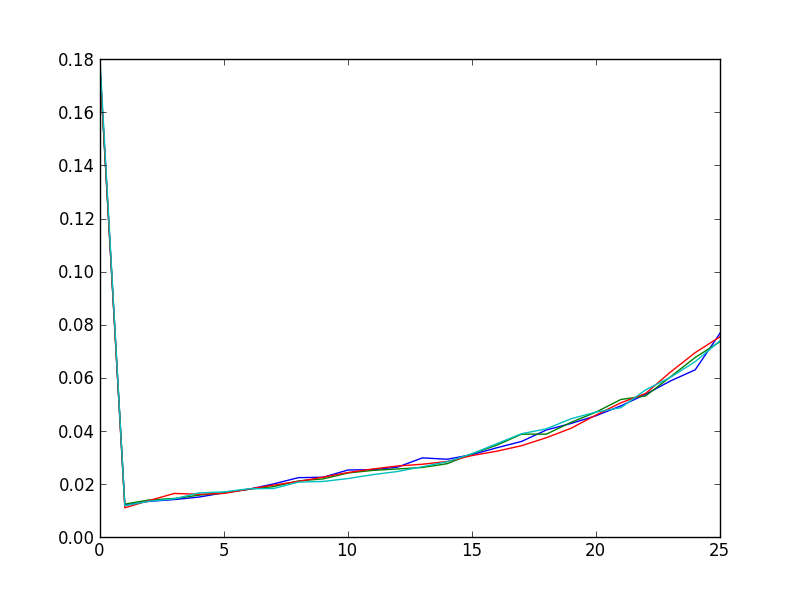
\includegraphics[width=0.5\textwidth]{lamFifth}}
    ~
     \subfloat[$\lambda=1/5,\alpha=15$]{\label{fig:lamFifth2}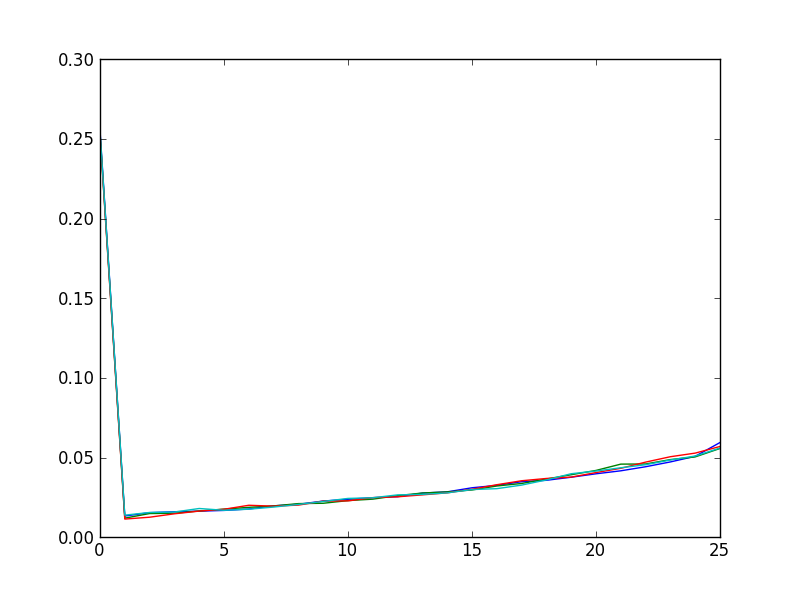
\includegraphics[width=0.5\textwidth]{lamFifth2}}
  \caption{Comparing different $\alpha$}
\end{figure}
Figure 1 plots the probabilities of each queue having either 0, 1,..., 25 carts in it for each of the queues (given as different colors). We notice a spike at 0 when $\alpha=15$, which gives us that $P(|Q_i|=0)>P(|Q_i|=j)$ for every $j\in\{1,...,25\}$. The point here is that even though the cumulative probability of having at least one cart in each queue is greater than zero, there is still a high possibility of having zero carts (at least 20\% chance). However, since we are only running simulations based on arbitrary values, the real optimization can occur when someone collects actual data to determine the arrival and departure rates of carts from home and inputs them into this program, along with the number of carts and queues they currently have. 

In the case for $\gamma=25,\gamma=20$, we find that a good value for $\lambda$ is 1/3 since the $P(|X|>0)$ is seemingly maximized as its upper and lower bounds are maximized with the constraint that $\lambda$ be as small as possible. In other words, if on average the workers were to collect carts once every three hours and return them in batches, then the chances of home always having at least some carts increases dramatically, compared to the previous section where there were no batch returns. 

\section*{Conclusion}

The purpose of this project was more or less exploratory in nature rather than computationally intensive since I wanted to think about a problem that seemed interesting when I'd once visited a supermarket. Of course, there have been a lot of things I could have included or developed such as the inclusion of 'peak-time' shopping hours (where arrival and departure rates of carts increase over the course of a few hours every 3 or 4 hours), and to actually simulate customers that walk into a supermarket with a newly departed cart, take their time to shop, and enter a queue themselves for checkout which would add another component of randomness and change the arrival times of the carts, resulting in a more realistic representation of $P(|X|>0)$. This would of course aid in finding the optimal solution as we have done, but in a more complete and possibly realistic manner.

\pagebreak
\section*{Appendix}
\subsection*{Part A: Python Code for Data Structures Used}
Here we define the cart object as a Node in Python from node.py:

\begin{singlespace}
\begin{verbatim}
class Node:
    '''
    Define the Node class as shopping carts.
    '''
    
    def __init__(self, i=0, j=0, timestamp=0, returnt=0, out=False):
        '''
        Constructor for the Node class.
        '''
        self.i = i
        self.j = j
        self.timestamp = timestamp
        self.returnt = returnt
        self.out = out
        
    def __cmp__(self, other):
        '''
        Compare equality of nodes by checking if same indices, otherwise return
        False.
        '''
        if self.i == other.i and self.j == other.j:
            return 0
        else:
            return -1
        #We will only ever use the inequality since greater or less than does 
        # not make any sense for our purposes.
    
    def __str__(self):
        '''
        Return a string representation of node object.
        '''
        s = '[i:' + str(self.i) + ', j:' + str(self.j) + ', timestamp:' + \
          str(self.timestamp) + ', returnt:' + str(self.returnt) + ', out:' + \
          str(self.out) + ']'
        return(str(s))

\end{verbatim}
\end{singlespace}
\pagebreak

Here we define the Stack object (i.e. Queue objects) used for home (X), Out, and Aban in Queue.py:
\begin{singlespace}
\begin{verbatim}
from node import *

class Queue:
    '''
    Define a Queue ADT with a LIFO structure.
    '''
    
    def __init__(self):
        '''
        Constructor for Queue data type with initialized empty list.
        '''
        self.queue = []
        
    def __str__(self):
        '''
        String reperesentation of Queue object.
        '''
        if self.queue == []:
            return '{}'
        s = '{'
        for item in self.queue:
            s += str(item) + ', '
        s = s[:-2] + '}'
        return s
        
    def push(self, cart):
        '''
        Push a new element at the end of the queue.
        '''
        self.queue.append(cart)
        
    def size(self):
        '''
        Get length of the queue.
        '''
        return(len(self.queue))
        
    def pop(self):
        '''
        Pop the end of the queue (FILO)
        '''
        x = self.queue[-1]
        self.queue = self.queue[:-1]
        return(x)
    
    def remove(self, n):
        '''
        Remove the item at index n, n in 0 to len(self.queue)-1.
        '''
        if n < self.size():
            x = self.queue[n]
            self.queue = self.queue[:n] + self.queue[n+1:]
            return x
    
    def get_ind(self, node):
        '''
        Return the index of the node in Queue.
        '''
        count = 0
        for item in self.queue:
            if node == item:
                return count
            count += 1
\end{verbatim}
\end{singlespace}

Here we define the class for home (X) with its methods in Queue.py:
\begin{singlespace}
\begin{verbatim}
class Matrix:
    '''
    The class for a list of Queue objects (i.e. our trolley database).
    '''
    
    def __init__(self, N=0, M=0):
        '''
        Constructor to initialize N Queues each with M nodes.
        '''
        d = {}
        for k in range(1, N+1):
            d[k] = Queue()                  #Create dictionary of queues with
            for l in range(1, M+1):         # queue number as key
                d[k].push(Node(i=k, j=l))
        self.d = d
    
    def __str__(self):
        '''
        String representation of Matrix.
        '''
        if self.d.keys() == []:
            return '{}'
        else:
            s = '{'
            for item in self.d.keys():
                s += str(self.d[item]) + '\n'
            s = s + '}'
            return s
    
    def pop(self, lst):
        '''
        Pop the last element of the queue indexed at lst.
        '''
        car = self.d[lst].pop()
        car.out = True
        return car

    def push(self, lst, cart):
        '''
        Push the node object cart into the Matrix object at queue indexed at
        lst.
        '''
        cart.out = False
        cart.timestamp = cart.returnt = 0
        self.d[lst].push(cart)
        
    def getsizes(self):
        m = {}
        for k in self.d.keys():
            m[k] = self.d[k].size()
        return m
\end{verbatim}
\end{singlespace}

\pagebreak
\subsection*{Part B: Python Code for Helper Functions}
Here we have with docstrings the helper functions used in Python from file helperfns.py:
\begin{singlespace}
\begin{verbatim}
from Queue import *
from node import *
import random
import operator

M = 25		#Number of trolleys in each queue
N = 4		#Number of queues
gamma = 30 	#Departure rate of carts per time period such that rho < 1
alpha = 15	#Arrival rate of carts per hour
lam = 0.5

def weighted_choice(weights): 
    '''
    Return an index from a list given the weights of said list. Courtesy of     
    http://eli.thegreenplace.net/2010/01/22/weighted-random-generation-in-python/#id4
    '''
    totals = []           
    running_total = 0
    for w in weights:
        running_total += w
        totals.append(running_total)

    rnd = random.random() * running_total
    for i, total in enumerate(totals):
        if rnd < total:
            return i

def outweights(out):
    '''
    Get weights for the Out Queue based on smallest return time being given
    the largest weight i.e. probability of returning.
    '''
    weights = [0]*out.size()
    if out.size() > 0:
        weights = [0]*out.size()
        m = 0
        for cart in out.queue:
            weights[m] = 1/cart.returnt
            m += 1
        weights = [x / sum(weights) for x in weights]
    return weights
    
def return_aban(Aban, X):
    '''
    Return all abandoned carts based on the weights given to the queues 
    in the cart database.
    '''
    if Aban.size() > 0:
        sizes = X.getsizes()
        sizes = sorted(sizes.iteritems(), key=operator.itemgetter(1))
          #Get sorted tuples based on number of elements in each queue,
          # from smallest to largest
        tofill = []
        for tup in sizes:
            x = (tup[0],tup[1],M-tup[1])
            tofill.append(x)
        for T in range(N):
            for S in range(tofill[T][2]):
                if Aban.size() > 0:
                    X.push(sizes[T][0], Aban.pop())
                                       
def newarrivaltime():
    return random.expovariate(alpha)

def newdeparturetime():
    return random.expovariate(gamma)

def newbatchreturntime():
    return random.expovariate(lam)

def depweight(Q):
    '''
    Compute weights for queues for departure of next trolley, Q is a list of
    trolley counts for X.
    '''
    if sum(Q) == 0:
        return Q
    return [(float(x)/sum(Q)) for x in Q]

def count_zero(Q):
    '''
    Return the count of items that happen to be zero in list Q.
    '''
    c = 0
    for i in range(len(Q)):
        if Q[i] == 0:
            c += 1
    return c

def count_M(Q):
    '''
    Return the count of items that happen to be M in list Q.
    '''
    c = 0
    for i in range(len(Q)):
        if Q[i] == M:
            c += 1
    return c

def arrweight(Q):
    '''
    Compute weights for queues for arrival of next trolley. Based on the
    assumption that queues with larger number of trolleys will usually
    get more trolleys due to convenience.
    '''
    l = len(Q)
    weights = [0.0]*l
    sumtot = 0
    for i in range(l):
        if Q[i] < M:
            weights[i] = Q[i]
            sumtot = sumtot + weights[i]
    if count_zero(Q) == l - count_M(Q):  
        #If queues only have lenghts 0 and M, give equal weight to those with 0
        for i in range(l):
            if Q[i] == 0:
                weights[i] = 1.0/count_zero(Q)
        return weights
    if sumtot == 0:
        return weights
    return [float(x)/sumtot for x in weights]

def getsortdict(d):
    '''
    Return a sorted list of values from dictionary d where sorting is based
    on the keys.
    '''
    Q = sorted(d.iteritems(), key=operator.itemgetter(0))
    Y = []
    for tup in Q:
        Y.append(tup[1])
    return Y
\end{verbatim}
\end{singlespace}
\pagebreak

\subsection*{Part C: Simulation Code for Non-Batches \& Batches}
The code for both batches and non-batches is essentially the same since we use a Boolean to indicate if batch arrivals are allowed to occur (i.e. non-batches is a special case of batches). Here is the code from simulation.py. Notice that it is heavily based on the code from Prof. Rosenthal's supplementary program Rqueue.
\begin{singlespace}
\begin{verbatim}
from helperfns import *
from pylab import *
import random
import operator
import numpy

rep = 5
probvec = []
for z in range(rep):
    #This loop is just for repeated simulations to check for consistency

    X = Matrix(N, M)  
        #The cart 'database' containing the queues for arrival and departure
    Out = Queue()     
        #Initialize an empty list to record all trolleys that are currently 
        # out but not abandoned
    Aban = Queue()    
        #Initialize an empty list of trolleys that have been abandoned 
        #(when return time has expired)
    
    TARGETTIME = 10000
    MAXGRAPH = M 
    dobatches = False
    timetodepart = newdeparturetime() 
    timetoarrive = 0 
    timeremaining = TARGETTIME 
    nextbatchtime = [newbatchreturntime(), timeremaining]
    thetimesQ = {}
    trace = []
    for i in range(1,N+1):
        thetimesQ[i] = [0]*(M+1)
    

    while timeremaining > 0:
        
        if Aban.size() > 0 and nextbatchtime[1] - timeremaining > nextbatchtime[0]\
           and dobatches:
            #We will now return all the abandoned trolleys to the queues
            return_aban(Aban, X)
            nextbatchtime = [newbatchreturntime(), timeremaining]
        
        if timeremaining <= timetodepart and timeremaining <= timetoarrive:
            # Finish without any further events.
            get = X.getsizes()        
            for i in range(1, N+1):
                if get[i] <= MAXGRAPH:
                    thetimesQ[i][get[i]] += timeremaining
            timeremaining = 0
        elif sum(X.getsizes().values()) == 0 or timetodepart < timetoarrive:
            # Await next trolley departure.
            timeremaining = timeremaining - timetodepart
            timetoarrive = timetoarrive - timetodepart
            get = X.getsizes()        
            for i in range(1, N+1):
                if get[i] <= MAXGRAPH:
                    thetimesQ[i][get[i]] += timetodepart
            if sum(X.getsizes().values()) > 0:       
                # there are trolleys still in the queues
                timetoarrive = newarrivaltime()
                Q = X.getsizes()
                Q = getsortdict(Q)
                dchosen = weighted_choice(depweight(Q))
                #Q[dchosen] -= 1
                cart = X.pop(dchosen+1)
                cart.returnt = timetoarrive
                cart.timestamp = timeremaining
                Out.push(cart)
                trace.append(sum(X.getsizes().values()))
            timetodepart = newdeparturetime()
        else:    
            # Await next trolley arrival.
            timeremaining = timeremaining - timetoarrive
            timetodepart = timetodepart - timetoarrive
            get = X.getsizes()        
            for i in range(1, N+1):
                if get[i] <= MAXGRAPH:
                    thetimesQ[i][get[i]] += timetoarrive
            if sum( X.getsizes().values()) < N*M and Out.size() > 0:
                Q = X.getsizes()
                Q = getsortdict(Q)            
                achosen = weighted_choice(arrweight(Q))
                w = outweights(Out)
                cart = Out.remove(weighted_choice(w))
                X.push(achosen+1, cart)
                trace.append(sum(X.getsizes().values()))
            timetoarrive = newarrivaltime()
        if Out.size() > 0 and dobatches:
            for item in Out.queue:
                if item.timestamp - timeremaining > item.returnt:
                    m = Out.get_ind(item)
                    Aban.push(Out.remove(m))
            trace.append(sum(X.getsizes().values()))
                
    #print X.getsizes()
    #print thetimesQ
    thefracs = {}
    for i in thetimesQ.keys():
        thefracs[i] = [x/TARGETTIME for x in thetimesQ[i]]
    #print thefracs
    #x = arange(0,M+1,1)
    #for j in thefracs.keys():
    #    plot(x, thefracs[j])
    y = arange(0,len(trace),1)
    plot(y,trace)
        
    #Computing P(|Q_j|>0):
    theprobs = [0]*N
    for i in range(1, N+1):
        theprobs[i-1] = sum(thefracs[i][1:])
    probvec.append(theprobs)
    
J = numpy.array(probvec)
Jmean = numpy.mean(J, axis = 0)
    #Get mean across columns (i.e. between runs, not within runs)
Jstd = numpy.std(J, axis = 0)
    #Get standard error across columns (i.e. between runs, not within runs)

\end{verbatim}
\end{singlespace}
\pagebreak

\subsection*{Part D: Some Figures of Interest}

\begin{figure}[h!]
  \centering
    \subfloat[$\gamma=20,\alpha=20$]{\label{fig:alpha20gamma20}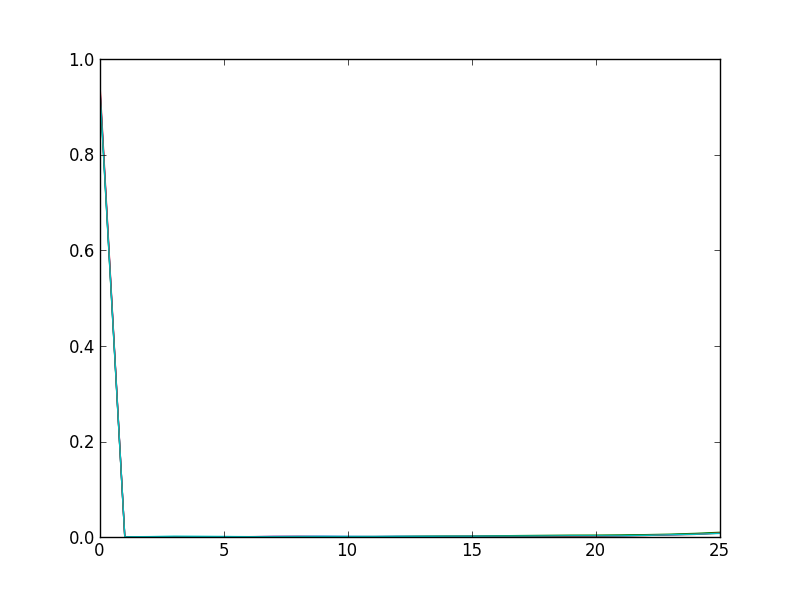
\includegraphics[width=0.5\textwidth]{alpha20gamma20}}
    ~
     \subfloat[Tracing $|X|$ over Time]{\label{fig:alpha20gamma20trace}\includegraphics[width=0.5\textwidth]{alpha20gamma20trace}}
  \caption{Row 1 of Table 1}
\end{figure}

\begin{figure}[h!]
  \centering
    \subfloat[$\gamma=25,\alpha=20$]{\label{fig:alpha20gamma25}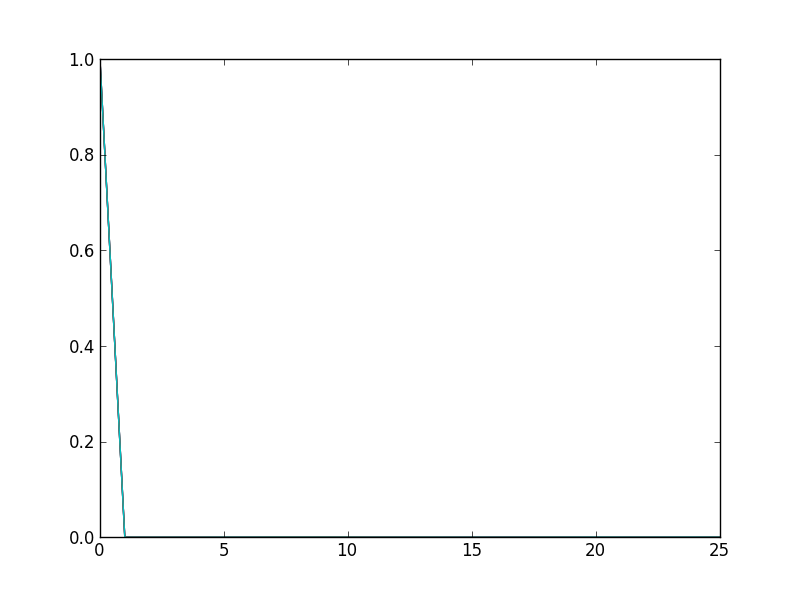
\includegraphics[width=0.5\textwidth]{alpha20gamma25}}
    ~
     \subfloat[Tracing $|X|$ over Time]{\label{fig:alpha20gamma25trace}\includegraphics[width=0.5\textwidth]{alpha20gamma25trace}}
  \caption{Row 2 of Table 1}
\end{figure}

\begin{figure}[h!]
  \centering
     \subfloat[Tracing $|X|$ over Time]{\label{fig:M40trace}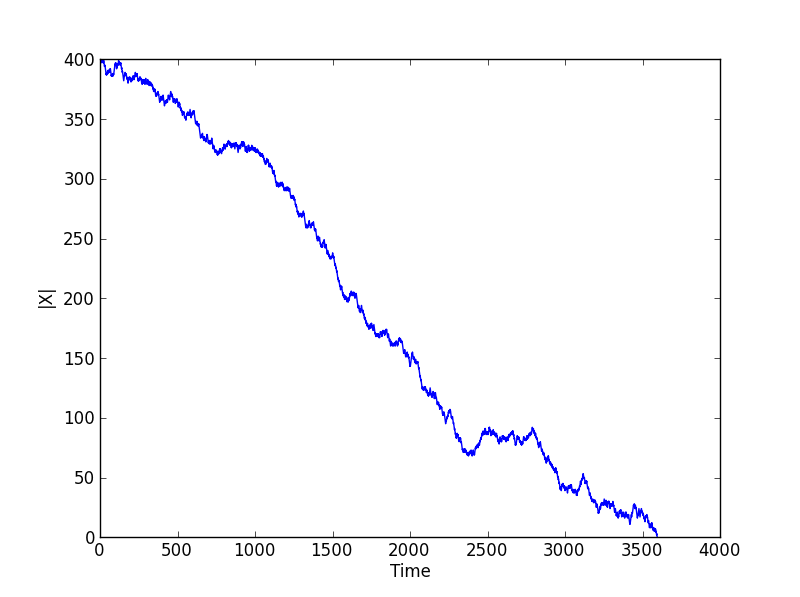
\includegraphics[width=0.5\textwidth]{M40trace}}
  \caption{Row 4 of Table 1}
\end{figure}
\end{document}
